\documentclass{article}

\usepackage{cancel}
\usepackage{tikz}
\usepackage{amsmath}
\usepackage{geometry}
\usepackage{graphicx}
\usepackage{amsfonts} 
\usepackage{verbatim}
\usepackage{mathrsfs}  
\usepackage{lmodern}
\usepackage{braket}
\usepackage{hyperref}

\hypersetup{
    colorlinks=true,
    linkcolor=black,
}

\renewcommand{\contentsname}{Indice}

\tikzset{sum/.style= {draw, fill=white, very thick, circle, node distance=0.5cm}}
\numberwithin{equation}{subsection}

\title{Appunti di Elettrotecnica ed Elettronica}
\author{Giacomo Sturm}
\date{AA: 2023/2024 - Ing. Informatica}

\begin{document}

\maketitle

\vspace{10mm}

\begin{center}
    Sorgente del file LaTeX disponibile su \url{https://github.com/00Darxk/Elettrotecnica-ed-Elettronica}
\end{center}

\clearpage

\tableofcontents

\clearpage

\section{Introduzione: Elementi di Fisica}

\subsection{Forza Elettrica}
Le prime analisi documentate sugli effetti elettrici risalgono agli antichi greci, da cui deriva il nome "electron"; $\eta\lambda\varepsilon\kappa\tau\rho o\nu$ in greco. Letteralmente significa ambra, poiché 
quando viene sfregata contro della lana, è capace di attrarre materiali, ovvero è in grado di generare un campo elettrico.

La forza elettrica venne analizzata da Coulomb in maniera simile all'analisi di Newton sulla gravità, poiché le due forze presentano dei comportamenti simili. La forza di 
gravità è una forza attrattiva tra due masse nello spazio, per cui sono presenti due forze applicate ad entrambe le masse di modulo e direzione uguale, ma verso opposto: 
\begin{equation*}
    \vec{F}_{1\to2}=G\displaystyle\frac{m_1m_2}{r^2}\hat{r}_{1\to2}=-\vec{F}_{2\to1}
\end{equation*}
Analogamente la forza elettrica è presente solo nell'interazione tra due elementi dotati di una carica che può presentarsi in due classi diverse, per convezione 
positiva o negativa, vengono misurate in Coulomb $C$ nel SI. Due cariche appartenenti alla stessa classe si oppongono, mentre due cariche appartenenti a due classi diverse 
si attraggono:
\begin{gather}
    \vec{F}_{1\to2}=-k_0\displaystyle\frac{q_1q_2}{r^2}\hat{r}_{1\to2}=-\vec{F}_{2\to1}\\
    F=k_0\displaystyle\frac{|q_1q_2|}{r^2}
\end{gather} 
Viene chiamata $k_0$ costante elettrica nel vuoto. 


La forza di gravità è una forza solamente attrattiva e presenta una sola classe di masse a differenza della forza elettrica. Poiché la forza di gravità si 
presenta solamente dall'interazione tra due masse, una massa singola nello spazio non è soggetta a forze di gravità. Questa massa è pronta ad interagire con un eventuale 
seconda massa per comunicare tra di loro la massa deforma in qualche modo lo spazio. Convenzionalmente si considera una deformazione convessa nella zona di spazio dove 
si trova la massa: 
\begin{center}
    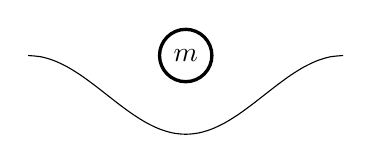
\begin{tikzpicture}[scale=2]
        \node[sum](o)at(0,0){$m$};
        \draw[-]plot[smooth, domain=-1:1](\x,{0.25*cos(180*(\x)-pi r)-0.25});
    \end{tikzpicture}
\end{center}

Poiché le cariche possono appartenere a due classi diverse per convenzione una carica positiva crea una deformazione concava, mentre una negativa una deformarzione convessa: 
\begin{center}
    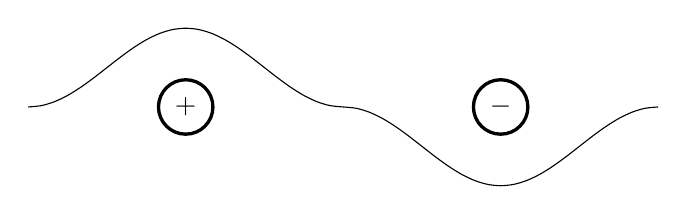
\begin{tikzpicture}[scale=2]
        \node[sum](o1)at(0,0){$+$};
        \draw[-]plot[smooth, domain=-1:1](\x,{-0.25*cos(180*(\x)-pi r)+0.25});
        
        \node[sum](o2)at(2,0){$-$};
        \draw[-]plot[smooth, domain=1:3](\x,{0.25*cos(180*(\x-2)-pi r)-0.25});
    \end{tikzpicture}
\end{center}
Per cui le cariche positive tendono a "scendere", mentre le cariche negative tendono a "salire". La deformazione spaziale è dovuta ad un campo gravitazionale o elettrico, 
dalle interazione del campo si genera una forza gravitazionale o elettrica. 

\subsection{Campo Elettrico}
Un campo elettrico $\vec{E}(x,y,z)$ è un campo vettoriale, ovvero è un insieme di vettori per ogni punto dello spazio dipendenti dalla loro posizione. Per misurare il campo 
generato da una carica $Q$ positiva per convenzione, si considera un'altra carica positiva $q<<Q$ usata per misurare la forza elettrica $\vec{F}$ generata dall'interazione con 
il campo $\vec{E}$. Si considera invece della costante elettrica nel vuoto $k_0$, la costante di permettività dielettrica nel vuoto $\varepsilon$:
\begin{gather}
    k_0=\displaystyle\frac{1}{4\pi\varepsilon_0},\:
    \varepsilon_0\approx8.86\times10^{-12}\left[\displaystyle\frac{C^2}{m^2}\frac{1}{N}\right]
\end{gather} 
Per misurare il campo elettrico in punto dello spazio di posizione $\vec{r}$ si considera la forza per unità di carica in quel punto:
\begin{equation}
    \vec{E}(x,y,z)=\displaystyle\frac{\vec{F}(x,y,z)}{q}=\frac{1}{4\pi\varepsilon_0}\frac{Q}{r^2}\hat{r}\left[\frac{N}{C}\right]
\end{equation}
Il campo elettrico generato da una singola carica puntiforme ha una direzione radiale e verso entrante se è una carica negativa ed uscente se si tratta di una carica positiva. 
Per indicare la direzione ed il verso di un campo vettoriale vengono usate linee di forza, la cui tangente in un punto rappresenta la direzione ed il verso del campo nello 
stesso punto. 
\begin{center}
    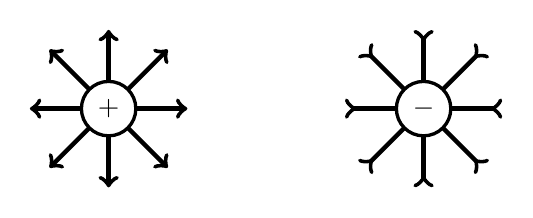
\begin{tikzpicture}[scale=2]
        \draw[<->, ultra thick](-0.5,0)--(0.5,0);
        \draw[>-<, ultra thick](1.5,0)--(2.5,0);

        \draw[<->, ultra thick](0,-0.5)--(0,0.5);
        \draw[>-<, ultra thick](2,-0.5)--(2,0.5);

        \draw[<->, ultra thick](-0.375,-0.375)--(0.375,0.375);
        \draw[<->, ultra thick](0.375,-0.375)--(-0.375,0.375);

        \draw[>-<, ultra thick](1.625,-0.375)--(2.375,0.375);
        \draw[>-<, ultra thick](2.375,-0.375)--(1.625,0.375);

        \node[sum](+)at(0,0){$+$};
        \node[sum](-)at(2,0){$-$};
    \end{tikzpicture}
\end{center}


In generale una forza elettrica è effetto dall'interazione di una carica $q$ con un campo elettrico $\vec{E}$, indipendentemente da ciò che genera il campo elettrico. Nel 
caso di una carica stazionaria o in moto rettilineo uniforme, si considera un campo elettro-stazionario, per cui la forza generata si esprime come il prodotto per la carica 
ed il campo elettrico: 
\begin{equation}
    \vec{F}=q\vec{E}
\end{equation}

L'unità di misura fondamentale usata per analizzare fenomeni elettrici nel SI è l'Ampere $A$, intensità di corrente, che ha sostituito il Coulomb $C$, unità di carica, 
entrambe sono cognomi di scienziati che hanno studiato l'elettricità, a differenza delle restanti grandezze fondamentali. Ciò spiega come non fosse chiaramanete 
idefntificabile la causa dei fenomeni elettrici in passato. 


In caso sia presente più di una carica stazionaria nel vuoto, per determinare il campo elettrico in un dato punto si considera il principio di sovrapposizione degli effetti 
(P.S.E.), applicabile solo in situazioni di tipo lineare, come nel vuoto essendo un elemento lineare. Per il principio della sovrapposizione degli effetti, il campo in un 
punto è dato dalla somma vettoriale di tutti i campi in quel punto, per cui i campi agiscono indipendentemente l'uno dall'altro. In una configurazione a due cariche, una 
positiva ed una negativa, il campo totale agente su una carica positiva posta in una posizione $P$ risulta essere: $\vec{E}_P=\vec{E}_1+\vec{E}_2$. 
\begin{center}
    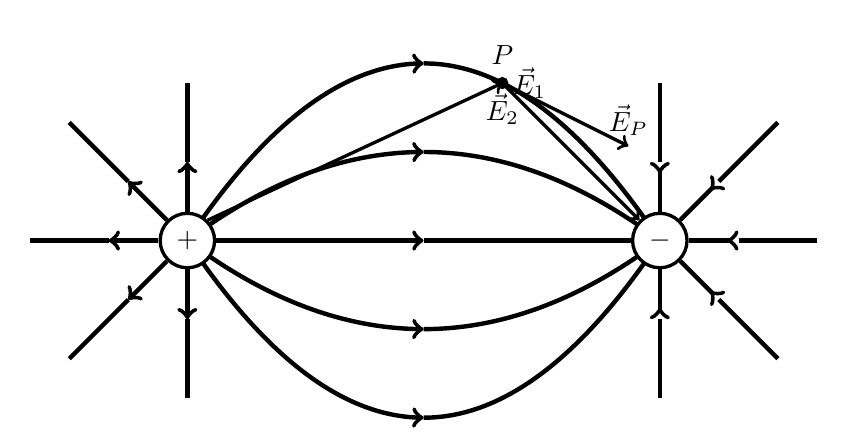
\begin{tikzpicture}[scale=2]
        \draw[->,ultra thick]plot[smooth, domain=0:1.5](\x,{0.25*(\x)*(\x-3)});
        \draw[-,ultra thick]plot[smooth, domain=1.5:3](\x,{(0.25*\x)*(\x-3)});

        \draw[->,ultra thick]plot[smooth, domain=0:1.5](\x,{-0.25*(\x)*(\x-3)});
        \draw[-,ultra thick]plot[smooth, domain=1.5:3](\x,{-0.25*(\x)*(\x-3)});

        \draw[->,ultra thick]plot[smooth, domain=0:1.5](\x,{0.5*(\x)*(\x-3)});
        \draw[-,ultra thick]plot[smooth, domain=1.5:3](\x,{(0.5*\x)*(\x-3)});

        \draw[->,ultra thick]plot[smooth, domain=0:1.5](\x,{-0.5*(\x)*(\x-3)});
        \draw[-,ultra thick]plot[smooth, domain=1.5:3](\x,{-0.5*(\x)*(\x-3)});

        \draw[<->,ultra thick](0,-0.5)--(0,0.5);
        \draw[ultra thick](0,-0.5)--(0,-1);
        \draw[ultra thick](0,0.5)--(0,1);

        \draw[>-<,ultra thick](3,-0.5)--(3,0.5);
        \draw[ultra thick](3,-0.5)--(3,-1);
        \draw[ultra thick](3,0.5)--(3,1);        

        \node[sum](+)at(0,0){$+$};
        \node[sum](-)at(3,0){$-$};

        \filldraw[circle](2,1)node[above]{$P$}circle(1pt);
        \draw[->,very thick](+.45)--(2,1)node[below]{$\vec{E}_2$};
        \draw[->,very thick](2,1)node[right]{$\vec{E}_1$}--(-.135);
        \draw[->,very thick](2,1)--(2.8,0.6)node[above]{$\vec{E}_P$};

        \draw[->, ultra thick](+.0)--(1.5,0);
        \draw[-,ultra thick](1.5,0)--(-.180);

        \draw[->,ultra thick](+.180)--(-0.5,0);
        \draw[ultra thick](-0.5,0)--(-1,0);
        \draw[-<,ultra thick](-.0)--(3.5,0);
        \draw[ultra thick](3.5,0)--(4,0);

        \draw[->,ultra thick](+.135)--(-0.375,0.375);
        \draw[->,ultra thick](+.225)--(-0.375,-0.375);
        \draw[-,ultra thick](-0.375,0.375)--(-0.75,0.75);
        \draw[-,ultra thick](-0.375,-0.375)--(-0.75,-0.75);

        \draw[-<,ultra thick](-.45)--(3.375,0.375);
        \draw[-<,ultra thick](-.315)--(3.375,-0.375);
        \draw[-,ultra thick](3.375,0.375)--(3.75,0.75);
        \draw[-,ultra thick](3.375,-0.375)--(3.75,-0.75);
    \end{tikzpicture}
\end{center}


Il campo elettrico stazionario, come il campo gravitazionale, è conservativo, per cui il lavoro svolto equivale all'opposto della differenza di energia potenziale. Per 
convenzione lo stato di riferimento dell'energia potenziale elettrica si trova ad una distanza infinita dalla carica, per cui l'energia corrisponde al lavoro necessario per 
spostare una carica $q$ da una distanza infinita ad una distanza finita $R$ da un campo elettrico $\vec{E}$. Si considera una campo elettrico generato da una carica puntiforme 
$Q$:
\begin{gather*}
    \Delta U(r)=-L=-\displaystyle\int_{+\infty}^R\vec{F}\cdot d\vec{r}\\
    \displaystyle\int_{+\infty}^Rq\vec{E}\cdot d\vec{r}=\int_{+\infty}^R\frac{1}{4\pi\varepsilon_0}\frac{qQ}{r^2}\cancelto{1}{\hat{r}\cdot \hat{r}}dr\\
    \cancelto{0}{-\displaystyle\frac{1}{4\pi\varepsilon_0}\frac{qQ}{+\infty}}+\frac{1}{4\pi\varepsilon_0}\frac{qQ}{R}
\end{gather*}
\begin{equation}
    U(r)=\frac{1}{4\pi\varepsilon_0}\frac{qQ}{R}=-L(r)
\end{equation}


Viene definito il potenziale elettrico $V$ il lavoro per unità di carica, viene misurato nel SI in Volt $V$:
\begin{equation}
    \Delta V=\displaystyle-\frac{L}{q}=-\int\frac{\vec{F}}{q}\cdot d\vec{r}=-\int\vec{E}\cdot d\vec{r}
\end{equation}
Corrisponde ad un integrale di linea del campo elettrico $\vec{E}$. 
Per un campo elettrico stazionario generato da una carica puntiforme $Q$ corrisponde a:
\begin{equation}
    V=\displaystyle\frac{1}{4\pi\varepsilon_0}\frac{Q}{R}\:\left[V\right]=\left[\frac{mN}{C}\right]
\end{equation}

In forma differenziale, il potenziale elettrico corrisponde a:
\begin{equation*}
    dV=-\vec{E}\cdot d\vec{r}=-(E_xdx+E_ydy+E_zdz)
\end{equation*}
Il differenziale $dV$ è un differenziale totale di un campo scalare $V(x,y,z)$, per cui corrisponde alla somma delle variazioni su ogni coordinata del differenziale della stessa: 
\begin{equation*}
    dV=\displaystyle\frac{\partial V}{\partial x}dx+\frac{\partial V}{\partial y}dy+\frac{\partial V}{\partial z}dz
\end{equation*}
Per il principio di indentità dei polinomi risulta:
\begin{equation*}
    \displaystyle\frac{\partial V}{\partial x}=-E_x,\:\frac{\partial V}{\partial y}=-E_y,\:\frac{\partial V}{\partial z}=-E_z
\end{equation*}

Si considera l'operatore differenziale vettoriale nabla: 
\begin{equation*}
    \vec{\nabla}:=\left(\displaystyle\frac{\partial}{\partial x},\,\frac{\partial}{\partial y},\,\frac{\partial}{\partial z}\right)
\end{equation*}
Per cui è possibile esprimere la relazione tra il potenziale elettrico ed il campo elettrico considerando l'operazione di gradiente su un campo scalare $\vec{\nabla}V$: 
\begin{equation}
    \vec{E}=-\vec{\nabla}V
\end{equation}
La capacità di un campo di ammettere un potenziale è una condizione sufficiente della conservatività di un campo vettoriale. Un'altra condizione sufficiente dipende dal 
risultato della circuitazione del campo, ovvero l'integrale di linea su un qualsiasi percorso chiuso $\lambda$ del campo $\vec{E}$. Se la circuitazione del campo è nulla, 
allora il campo in questione è conservativo:
\begin{equation}
    \Gamma_\lambda(\vec{E})=\displaystyle\oint_{\lambda}\vec{E}\cdot d\vec{\lambda}=0
\end{equation}
Se il campo non è conservativo, implica che il campo è variabile per cui la circuitazione risulta diversa da zero. 


Oltre all'operazione di gradiente su un campo scalare, se si considera un campo vettoriale $\vec{a}(x,y,z)$, si possono definire altre due operazioni: la divergenza ed il 
rotore. La divergenze è definita come il prodotto scalare tra l'operatore nabla ed il campo $\vec{a}$:
\begin{gather*}
    \vec{\nabla}\cdot\vec{a}=\displaystyle\left(\frac{\partial}{\partial x}\hat{x}+\frac{\partial}{\partial y}\hat{y}+\frac{\partial}{\partial z}\hat z\right)\cdot\left(a_x\hat{x}+a_y\hat{y}+a_z\hat{z}\right)\\
    \displaystyle\frac{\partial a_x}{\partial x}\cancelto{1}{\hat{x}\cdot\hat{x}}+\frac{\partial a_y}{\partial x}\cancelto{0}{\hat{y}\cdot\hat{x}}+\frac{\partial a_z}{\partial x}\cancelto{0}{\hat{z}\cdot\hat{x}}+
    \frac{\partial a_x}{\partial y}\cancelto{0}{\hat{x}\cdot\hat{y}}+\frac{\partial a_y}{\partial y}\cancelto{1}{\hat{y}\cdot\hat{y}}+\frac{\partial a_z}{\partial y}\cancelto{0}{\hat{z}\cdot\hat{y}}+
    \frac{\partial a_x}{\partial z}\cancelto{0}{\hat{x}\cdot\hat{z}}+\frac{\partial a_y}{\partial z}\cancelto{0}{\hat{y}\cdot\hat{z}}+\frac{\partial a_z}{\partial z}\cancelto{1}{\hat{z}\cdot\hat{z}}
\end{gather*}
\begin{equation}
    \vec{\nabla}\cdot\vec{a}=\displaystyle\frac{\partial a_x}{\partial x}+\frac{\partial a_y}{\partial y}+\frac{\partial a_z}{\partial z}
\end{equation}
Il rotore è definito come il prodotto vettoriale tra l'operatore nabla ed il campo $\vec{a}$:
\begin{gather*}
    \vec{\nabla}\times\vec{a}=
    \begin{vmatrix}
        \hat{x} & \hat{y} & \hat{z} \\
        \displaystyle\frac{\partial}{\partial x} & \displaystyle\frac{\partial}{\partial y} & \displaystyle\frac{\partial}{\partial z}\\
        a_x & a_y & a_z
    \end{vmatrix}=
    \begin{vmatrix}
        \displaystyle\frac{\partial}{\partial y} & \displaystyle\frac{\partial }{\partial z}\\
        a_y & a_z
    \end{vmatrix}\hat{x}-
    \begin{vmatrix}
        \displaystyle\frac{\partial}{\partial x} & \displaystyle\frac{\partial}{\partial z}\\
        a_x & a_z
    \end{vmatrix}\hat{y}+
    \begin{vmatrix}
        \displaystyle\frac{\partial}{\partial x} & \displaystyle\frac{\partial}{\partial y}\\
        a_x & a_y
    \end{vmatrix}\hat{z}
\end{gather*}
\begin{equation}
    \vec{\nabla}\times\vec{a}=\left(\displaystyle\frac{\partial a_z}{\partial y}-\frac{\partial a_y}{\partial z}\right)\hat{x}-\left(\frac{\partial a_x}{\partial z}-\frac{\partial a_z}{\partial x}\right)\hat{y}+\left(\frac{\partial a_y}{\partial x}-\frac{\partial a_x}{\partial y}\right)\hat{z}
\end{equation}

\subsubsection{Teorema di Gauss}

\begin{quotation}
    Il flusso totale, entrane o uscente, del campo elettrico $\vec{E}$ generato da cariche interne ad una qualsiasi superficie chiusa $S$, attraverso 
    la stessa superficie equivale al rapporto tra la carica totale e la costante di permettività dielettrica nel vuoto $\varepsilon_0$:
    \begin{equation}
        \Phi_{S}(\vec{E})=\displaystyle\frac{Q}{\varepsilon_0}
    \end{equation}
\end{quotation}


Analogamente alla portata di un liquido attraverso una superficie, il flusso $\Phi$ di un campo vettoriale $\vec{v}$ determina l'intensità del campo attraverso una data superficie $S$. 
\begin{center}
    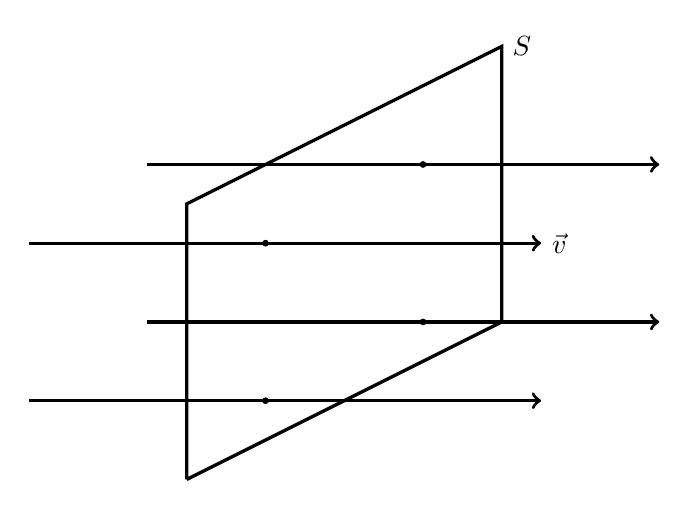
\begin{tikzpicture}[scale=2]
        \draw[very thick](0,0)--(0,1.75)--(2,2.75)node[right]{$S$}--(2,1)--(0,0);
        
        \draw[->,very thick](-1,0.5)--(2.25,0.5);
        \draw[->,very thick](-0.25,1)--(3,1);
        \draw[->,very thick](-1,1.5)--(2.25,1.5)node[right]{$\vec{v}$};
        \draw[->,very thick](-0.25,2)--(3,2);

        \filldraw[black](0.5,0.5)circle(0.5pt);
        \filldraw[black](1.5,1)circle(0.5pt);
        \filldraw[black](0.5,1.5)circle(0.5pt);
        \filldraw[black](1.5,2)circle(0.5pt);
    \end{tikzpicture}
\end{center}
Il flusso è massimo quando il campo e la superficie sono tra di loro perpendicolari: $\Phi_S(\vec{v})=|\vec{v}|\cdot S$. Per determinare il flusso attraverso una superfecie $S$ 
inclinata rispetto al campo $\vec{v}$ bisogna considerare la componente del campo che passa perpendicolarmente attraverso la superficie, per cui si definisce il versore 
giuntura di una superficie $\hat{n}_S$ come il vettore di modulo unitario, direzione normale alla superficie nel punto e di verso uscente se la superficie è concava, ed 
entrante se è convessa: $\Phi_S(\vec{v})=\vec{v}\cdot\hat{n}S$. 
In caso la superficie sia ondulata, la giacitura cambierebbe in base alla sua posizione, per cui per determinarne il flusso si considera un'approssimazione tramite la somma 
di flussi dello stesso campo attraverso suddivisioni della superficie, ognuna con una giacitura diversa: 
$\Phi_S(\vec{v})\approx\sum_{i=1}^N\vec{v}\cdot\hat{n}_iS_i$. Al diminuire della superficie $S_i$, la precisione aumenta, per cui per una superficie infinitesima si può 
determinare esattamente l'infinitesimo di flusso attraverso l'intera superficie: $\Phi_{dS}(\vec{v})=\vec{v}\cdot\hat{n}dS=d\Phi_{S}(\vec{v})$. In caso le suddivisioni 
siano finite, il flusso viene calcolato tramite una sommatoria, altrimenti per suddivisioni infinite si considera un integrale chiuso sulla superficie totale $S$:
\begin{equation}
    \displaystyle\Phi_S(\vec{v})=\oint_{S}\vec{v}\cdot\hat{n}dS
\end{equation}




Nel caso del teorema di Gauss, si considera una situazione semplificata, dove è presenta una singola carica $Q$ nel centro di una superficie sferica $S$ di raggio $r$. 
Considerando una sezione infinitesima della superficie $dS$, il versore giacitura $\hat{n}$ risulta essere sempre parallelo al campo elettrico $\vec{E}$ generato dalla carica, 
poiché si trova nel centro della sfera. Per cui il campo elettrico passante per ogni sezione infinitesima è costante, considerando l'integrale del flusso: 
\begin{gather*}
    \Phi_S(\vec{E})=\displaystyle\oint_{S}E\cancelto{1}{\hat{r}\cdot\hat{n}}dS=\oint_S\frac{Q}{4\pi\varepsilon_0r^2}dS=\frac{Q}{4\pi\varepsilon_0r^2}\oint_SdS=\frac{Q}{4\pi\varepsilon_0r^2}4\pi r^2
\end{gather*} 
\begin{equation}
    \Phi_S(\vec{E})=\frac{Q}{\varepsilon_0}
\end{equation}
\begin{center}
    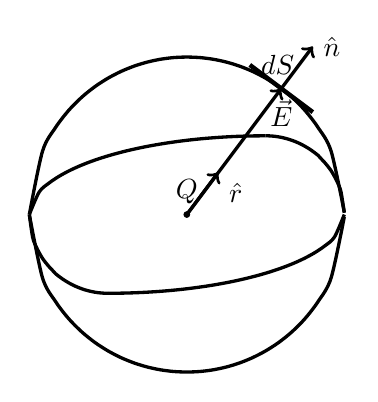
\begin{tikzpicture}[scale=2]
        \draw[-, very thick]plot[smooth, domain=-1:1](\x, {(1-(\x)^2)^0.5});
        \draw[-, very thick]plot[smooth, domain=-1:1](\x, {-(1-(\x)^2)^0.5});
        \draw[-, very thick]plot[smooth, domain=0.5:1](\x,{(0.25-(\x-0.5)^2)^0.5});
        \draw[-, very thick]plot[smooth, domain=-1:-0.5](\x,{-(0.25-(\x+0.5)^2)^0.5});
        \draw[-, very thick]plot[smooth, domain=-1:0.5](\x,{1/3*(2.25-(\x-0.5)^2)^0.5});
        \draw[-, very thick]plot[smooth, domain=-0.5:1](\x,{-1/3*(2.25-(\x+0.5)^2)^0.5});

        \filldraw[black](0,0)circle(0.5pt);

        \draw[->, very thick](0,0)node[above]{$Q$}--(0.6,0.8)node[below]{$\vec{E}$};
        \draw[->,very thick](0,0)--(0.2,0.267)node[below right]{$\hat{r}$};

        \draw[-, ultra thick](0.4,0.95)node[right]{$dS$}--(0.8,0.65);
        \draw[->,very thick](0.6,0.8)--(0.8,1.067)node[right]{$\hat{n}$};
    \end{tikzpicture}
\end{center}

Ciò implica che il campo elettrico ammette l'esistenza di sorgenti singole. Infatti se una carica si trova all'interno di una superficie chiusa, tutte le linee di campo generate 
escono attraverso la superficie, mentre se la carica si trovasse all'esterno della superficie, tutte le linee di campo entranti sarebbero necessariamente anche uscenti, ed il 
flusso totale sarebbe dato dalla somma del flusso entrante e del flusso uscente risultando nullo. 

\subsubsection{I Legge di Maxwell}

Il flusso attraverso una superficie chiusa è dato dalla somma del flusso per ogni faccia della superficie. Considerando un cubo infinitesimo con faccie parallele ai piani 
cartesiani ed un campo elettrico $\vec{E}$ passante per quel cubo, si calcola il flusso totale sommando il flusso sulle sue sei faccie. 
\begin{center}
    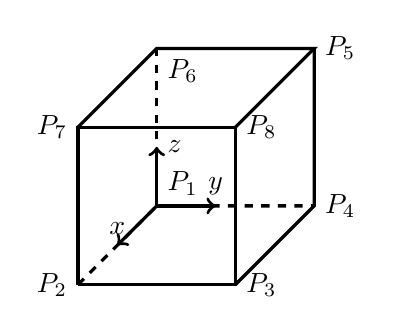
\begin{tikzpicture}[scale=2]
        \draw[-,very thick](0,0)node[left]{$P_2$}--(1,0)node[right]{$P_3$}--(1,1)node[right]{$P_8$}--(0,1)node[left]{$P_7$}--(0,0);
        \draw[dashed,very thick](0,0)--(0.5,0.5)node[above right]{$P_1$}--(1.5,0.5)node[right]{$P_4$};
        \draw[dashed,very thick](0.5,0.5)--(0.5,1.5)node[below right]{$P_6$};
        \draw[-,very thick](1,1)--(1.5,1.5)node[right]{$P_5$}--(0.5,1.5)--(0,1);
        \draw[-,very thick](1,0)--(1.5,0.5)--(1.5,1.5);
        \draw[->,very thick](0.5,0.5)--(0.25,0.25)node[above]{$x$};
        \draw[->,very thick](0.5,0.5)--(0.875,0.5)node[above]{$y$};
        \draw[->,very thick](0.5,0.5)--(0.5,0.875)node[right]{$z$};
    \end{tikzpicture}
\end{center}
\begin{align*}
    &P_1(x,y,z) &P_5(x,y+dy,z+dz)\\
    &P_2(x+dx,y,z) &P_6(x,y,z+dz)\\
    &P_3(x+dx,y+dy,z) &P_7(x+dx,y,z+dz)\\
    &P_4(x,y+dy,z) &P_8(x+dx,y+dy,z+dz)
\end{align*}

Il flusso attraverso la faccia $P_1P_2P_3P_4$ risulta essere:
\begin{equation*}
    \Phi_1(\vec{E})=\vec{E}\cdot\hat{n}dS=(E_x\cancelto{0}{\hat{x}\cdot\hat{n}}+E_y\cancelto{0}{\hat{y}\cdot\hat{n}}+E_z\cancelto{-1}{\hat{z}\cdot\hat{n}})dS=-E_zdxdy
\end{equation*}
Poiché il campo elettrico è antiparallelo alla giuntura della superficie. 


Consdierando la faccia $P_5P_6P_7P_8$, il campo elettrico varia prima di attraversare la faccia. La variazione dipende dalla variazione lungo l'asse $z$, per cui il cambiamento 
del campo elettrico dipende dalla sua derivata parziale $\displaystyle\frac{\partial\vec{E}}{\partial z}$. Il cambiamento effettivo è dato dalla derivata parziale 
moltiplicata per lo spostamento effettuato sull'asse $z$, trattandosi di un cubo infinitesimo lo spostamento è infinitesimo $dz$. Per cui il campo che attraversa la faccia 
risulta essere:
\begin{equation*}
    \vec{E}+\displaystyle\frac{\partial \vec{E}}{\partial z}dz
\end{equation*} 
Per cui il flusso risulta essere:
\begin{equation*}
    \Phi_2=\left(E_z+\displaystyle\frac{\partial E_z}{\partial z}dz\right)dxdy
\end{equation*}

Analogamente alla prima faccia, il flusso attraverso le due faccie $P_1P_2P_6P_7$ e $P_1P_4P_5P_6$ risultano essere:
\begin{gather*}
    \Phi_3=-E_ydxdz\\
    \Phi_5=-E_xdydz
\end{gather*}
Analogamente alla seconda faccia, il campo elettrico varia prima di attraversare le faccie $P_3P_4P_5P_8$ e $P_2P_3P_7P_8$, ed il loro flusso risulta essere:
\begin{gather*}
    \Phi_4=\left(E_y+\displaystyle\frac{\partial E_y}{\partial y}dy\right)dxdz\\
    \Phi_6=\left(E_x+\displaystyle\frac{\partial E_x}{\partial x}dx\right)dydz
\end{gather*}

Il flusso totale attraverso il cubo infinitesimo risulta quindi essere:
\begin{gather*}
    \Phi=\displaystyle\sum_{i=1}^6\Phi_i\\
    \begin{matrix}
        -E_zdxdy & -E_ydxdz & -E_xdydz\\
        +\left(E_z+\displaystyle\frac{\partial E_z}{\partial z}dz\right)dxdy & +\left(E_y+\displaystyle\frac{\partial E_y}{\partial y}dy\right)dxdz & +\left(E_x+\displaystyle\frac{\partial E_x}{\partial x}dx\right)dydz
    \end{matrix}\\
    \displaystyle\frac{\partial E_z}{\partial z}dxdydz+\frac{\partial E_y}{\partial y}dxdydz+\frac{\partial E_x}{\partial x}dxdydz\\
    \Phi=\left(\displaystyle\frac{\partial E_x}{\partial x}+\frac{\partial E_y}{\partial y}+\frac{\partial E_z}{\partial z}\right)dxdydz
\end{gather*}

Si cosidera il volume del cubo infinitesimo $d\tau=dxdydz$, mentre la superficie infinitesime che racchiude il volume $dS$. Il flusso attraverso il cubo equivale alla 
divergenza del campo elettrico: 
\begin{equation*}
    \Phi_{dS}(\vec{E})=\vec{\nabla}\cdot\vec{E}d\tau=d\Phi_S(\vec{E})
\end{equation*}
Per cui è possibile determinare il flusso di un campo elettrico (stazionario) $\vec{E}$ attraverso una superficie chiusa $S$, consideranro l'integrale sul volume 
racchiuso dalla superficie $\tau$ della divergenza del campo. Ciò viene chiamato teorema della divergenza. 
\begin{equation}
    \displaystyle\oint_S\vec{E}\cdot\hat{n}dS=\oint_{\tau}\vec{\nabla}\cdot\vec{E}d\tau
\end{equation} 
Per il teroema di Gauss il flusso di un campo elettrico $\vec{E}$ attraverso una qualsiasi superficie chiusa $S$ è dato dal rapporto delle carica totale $Q$ interna alla superficie 
e la permettività dielettrica nel vuoto $\varepsilon_0$. Dato un mezzo con densità uniforme di carica $\rho_Q$, la carica totale può essere espressa come l'integrale sull'intero 
volume della densità: 
\begin{equation*}
    Q=\displaystyle\oint_{\tau}\rho_Qd\tau
\end{equation*}  
Per il teorema di Gauss e per il teorema della divergenza:
\begin{gather*}
    \displaystyle\oint_{\tau}\vec{\nabla}\cdot \vec{E}d\tau=\oint_{\tau}\frac{\rho_Q}{\varepsilon_0}d\tau\\
    \vec{\nabla}\cdot\vec{E}=\displaystyle\frac{\rho_Q}{\varepsilon_0}
\end{gather*}

Viene definito vettore dello spostamento elettrico nel vuoto $\vec{D}:=\varepsilon_0\vec{E}$, per cui si può esprimere l'equazione precedente come:
\begin{equation}
    \vec{\nabla}\cdot\vec{D}=\rho_Q\,\displaystyle\left[\frac{Q}{m^3}\right]
\end{equation}
Questa è la prima legge di Maxwell in forma locale. 

\subsubsection{II Legge di Maxwell}

In un campo elettrico conservativo, la circuitazione lungo un qualsiasi percorso chiuso è nulla. Poiché il campo elettrico equivale all'inverso del gradiente del 
potenziale ed il potenziale è lavoro per unità di carica di un campo conservativo, su un percorso chiuso il lavoro è nullo, quindi anche la circuitazione. Esistono invece 
campi elettrici che non producono lavoro, ma forza elettro-motrice, per cui la circuitazione su un percorso chiuso è diversa da zero. 



Considerando una superficie quadrata infinitesima attraversata da un campo elettrico $\vec{E}$, si vuole calcolare la sua circuitazione, sommando la circuitazione sui suoi 
quattro lati infinitesimi, come il prodotto scalare tra il campo elettrico e lo spostamento $d\vec{\lambda}$. Per convenzione si considera una circuitazione positiva in senso 
antiorario. 
\begin{center}
    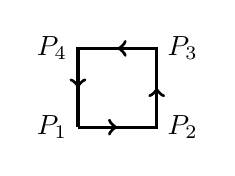
\begin{tikzpicture}
        \draw[-, very thick](0,0)node[left]{$P_1$}--(1,0)node[right]{$P_2$}--(1,1)node[right]{$P_3$}--(0,1)node[left]{$P_4$}--(0,0);
        \draw[->,very thick](0,0)--(0.5,0);
        \draw[->,very thick](1,0)--(1,0.5);
        \draw[->,very thick](1,1)--(0.5,1);
        \draw[->,very thick](0,1)--(0,0.5);
    \end{tikzpicture}
\end{center}
\begin{align*}
    &P_1(x,y,z)\\
    &P_2(x+dx,y,z)\\
    &P_3(x+dx,y+dy,z)\\
    &P_4(x,y+dy,z)
\end{align*}

Sul lato $P_1P_2$, il campo elettrico varia con l'aumento della coordinata $x$, poiché ogni componte del campo elettrico dipende dalle $3$ coordinate, la variazione di una 
coordinate implica una variazione di tutte le componenti del campo. La circuitazione risulta quindi essere:
\begin{equation*}
    \Gamma_1=\vec{E}\cdot d\vec{\lambda}=\left(E_x\hat{x}+\displaystyle\frac{\partial E_x}{\partial x}dx\hat{x}+E_y\hat{y}+\frac{\partial E_y}{\partial x}dy\hat{y}+E_z\hat{z}+\frac{\partial E_z}{\partial x}dz\hat{z}\right)\cdot d\vec{x}=\left(E_x+\frac{\partial E_x}{\partial x}dx\right)dx
\end{equation*}
Analogamente per il lato $P_2P_3$, il campo elettrico varia con l'aumento delle coordinata $x$ e $y$, per cui per ogni componente del campo sarà aggiunta una variazione dipendente 
dall'aumento delle $x$ e un'altra dall'aumento delle $y$:
\begin{equation*}
    \Gamma_2=\left(E_y\hat{y}+\displaystyle\frac{\partial E_y}{\partial x}dx\hat{y}+\frac{\partial E_y}{\partial y}dy\hat{y}\right)\cdot d\vec{y}=\left(E_y+\frac{\partial E_y}{\partial x}dx+\frac{\partial E_y}{\partial y}dy\right)dy
\end{equation*}

Per i lati $P_3P_4$ e $P_4P_1$ la direzione in cui vengono attraversati è opposta alla verso delle coordinate, per cui la circuitazione per questi lati è negativa:
\begin{gather*}
    \Gamma_3=-\left(E_x+\displaystyle\frac{\partial E_x}{\partial x}dx+\frac{\partial E_x}{\partial y}dy\right)dx\\
    \Gamma_4=-\left(E_y+\displaystyle\frac{\partial E_y}{\partial y}dy\right)dy
\end{gather*} 

La circuitazione totale risulta essere quindi:
\begin{gather*}
    \Gamma=\Gamma_1+\Gamma_2+\Gamma_3+\Gamma_4\\
    \begin{matrix}
        \displaystyle\left(E_x+\frac{\partial E_x}{\partial x}dx\right)dx+\left(E_y+\frac{\partial E_y}{\partial x}dx+\frac{\partial E_y}{\partial y}dy\right)dy\\
        \displaystyle-\left(E_x+\frac{\partial E_x}{\partial x}dx+\frac{\partial E_x}{\partial y}dy\right)dx-\left(E_y+\frac{\partial E_y}{\partial y}dy\right)dy
    \end{matrix}\\
    \Gamma=\left(\displaystyle\frac{\partial E_y}{\partial x}-\frac{\partial E_x}{\partial y}\right)dxdy
\end{gather*}
La circuitazione totale equivale alla componente del rotore del campo elettrico parallela alla normale al piano individuato dalla superficie descritta dal percorso $\lambda$. 
Poiché la circuitazione è uno scalare, per conservare solo questa componente si considera il prodotto scalare tra il rotore del campo elettrico ed il versore giacitura. 
Considerando il differenziale della superficie $dS=dxdy$, la circuitazione totale su una superficie infinetesimale è:
\begin{equation*}
    \Gamma_{d\lambda}=\vec{E}\cdot d\vec{\lambda}=(\vec{\nabla}\times\vec{E})\cdot \hat{n}dS=d\Gamma_\lambda
\end{equation*}
Integrando quest'ultima equazione si ottiene che la circuitazione per un qualsiasi percorso chiuso $\lambda$ di un campo elettrico (stazionario) $\vec{E}$ è esattamente il 
flusso del rotore del campo elettrico attraverso la superficie $S$ descritta dal quel percorso $\lambda$. Questo rappresenta il teorema del rotore: 
\begin{equation}
    \displaystyle\oint_{\lambda}\vec{E}\cdot d\vec{\lambda}=\oint_S(\vec{\nabla}\times\vec{E})\cdot\hat{n}dS
\end{equation}

Per il teroema della circuitazione ed il teorema del rotore, per tutti i campi conservativi, il rotore di un campo elettrico è nullo, condizione necessaria affinché un campo 
vettoriale sia conservativo: 
\begin{equation}
    \vec{\nabla}\times\vec{E}=\vec0
\end{equation}
Quest'equazione rappresenta la seconda equazione di Maxwell in forma stazionaria.

\subsection{Corrente e Magnetismo}

\end{document}